%The study of molecular and intermolecular structures and dynamics yield important insights about composition and alignment of materials as well as processes governing its properties.
%However, investigations on a molecular scale are limited mainly to spectroscopic methods where the system properties are obtained indirectly by measureing the interaction of the system under study with light, electron beams or other quantum particles.
%This yields a large variety of of spectroscopic methods that can be categorised by means of the incoming and outgoing particles.
Steady state as well as time-resolved photoelectron spec\-tros\-co\-py have become widely used tools to study the composition of gases and liquids \cite{winterWater,liquid1,XrayDynamics}, the structure of solids \cite{solid1} as well as chemical reactions such as electron transfer \cite{XrayDynamics}.
The process studied by photoelectron spectra is the absorption of a high-energetic photon (usually in the ultra-violet to hard X-ray regime) by an $N$-electron system which leads to the releas of an electron whose kinetic energy is measured.
This process is sketched in Figure \ref{fig:PESscheme} where the bound states are depicted by horizontal bars and the states of the outgoing electron are visualised by the gradient-filled block, indicating that its energy is continuous.
Measureing the kinetic energy of the photoelectron yields information on the energy of its previous states due to energy-conservation over the process.

One of the main reasons for the broad success of this particular type of spectroscopy is that these spectra are very sensitive to small changes in the chemical environment and hence yield information not only about the chemical structure of molecules but also about intermolecular interactions as for example solvation effects \cite{winterWater, solution1,solution2, solution3, solution4}.
\begin{wrapfigure}{r}{0.62\textwidth}
   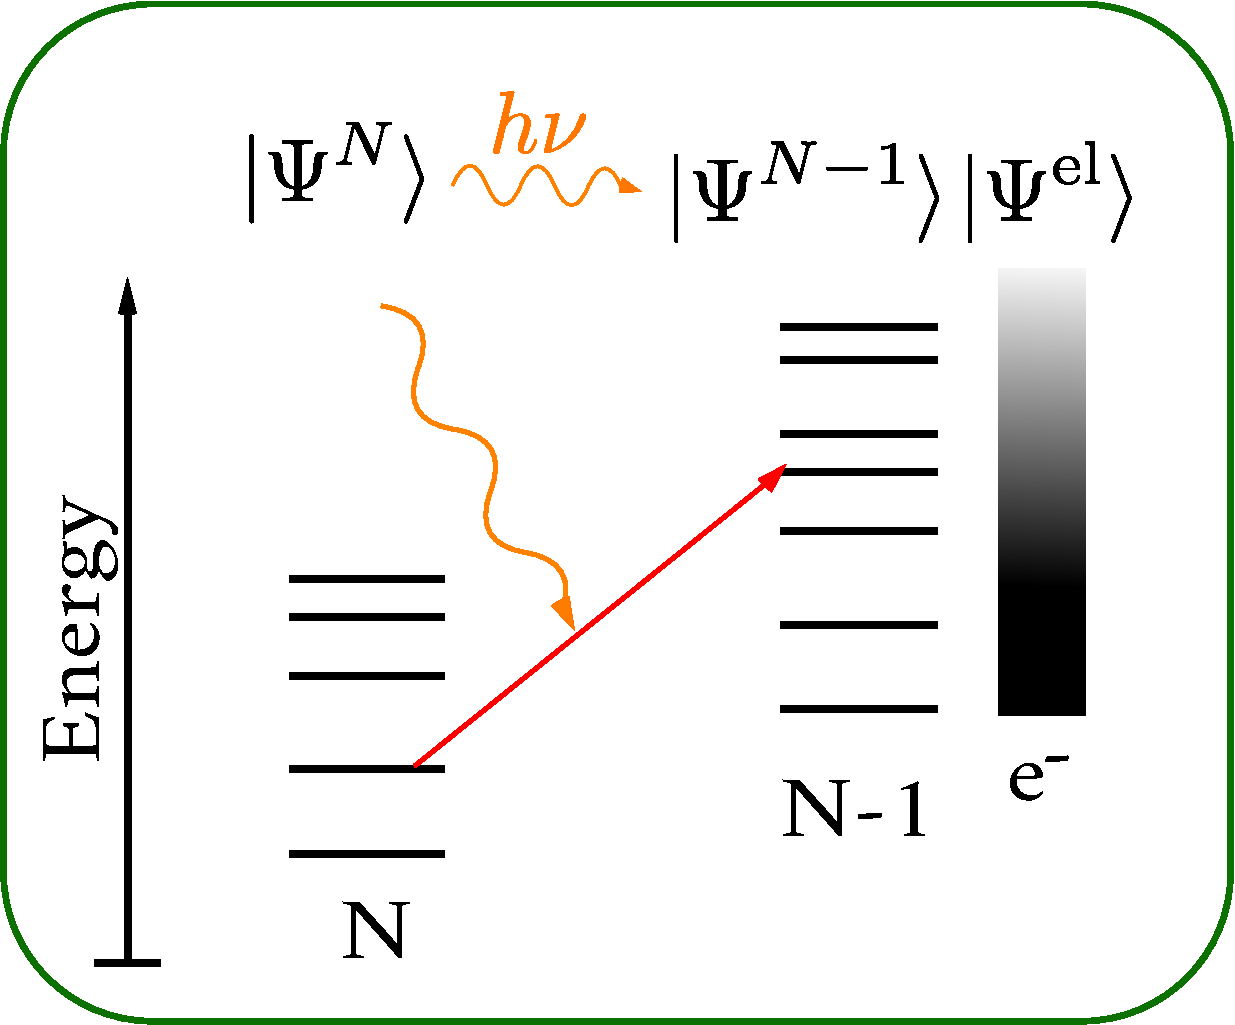
\includegraphics[width=0.61\textwidth]{Figures/PESscheme}
   \caption{Schematic representation of a photoelctron transition : an incoming photon with energy $h\nu$ ionises the $N$-electron system, transfering it into a free electron in a continuum state and a system of $N-1$ bound electrons.
   The bars denote bound states, the color-gradient depicts the energy of the outgoing electron.}
   \label{fig:PESscheme}
\end{wrapfigure}
Furthermore, photoelectron spectroscopy provides a more direct access to the energy levels than optical absorption and emission spectroscopy since the transition energies are obtained with respect to the vacuum level and no ``dark'' states occur due to different selection rules.
Finally the ease of handling changed particles experimentally makes this method appealing and a good temporal resolution can be achieved by varying the path in the time of flight spectrometer.
Moreover, besides its capabilities in steady state spectroscopy, photoelectron spectra are the standard tool to study attosecond physics due to the naturally high energy of the short pulses which ionise the systems under study \cite{as1, as2, as3, as4, as5, as6}.
However, a limitation of photoelectron spectroscopy is that the short free-path of electrons in condensed phases limits the probe depth significantly.

Having performed a measurement of a photoelectron spectrum (PES) it is, at least for complex systems, rich of features and hence the interpretation requires theoretical methods.
This especially applies to systems with strong electron correlation which manifests itself in the appearance of combination transitions.
Over the decades a large variety of methods to calculate photoelectron spectra have been developed at different levels of theory.
In literature often the theoretical spectra are estimated on the basis of Koopmans' theorem \cite{koopmans}, (or its density functional theory (DFT) counterpart \cite{koopmansDFT},) assuming equal intensities for all transitions \cite{OT-RSH,Koerzd1,Koerzd2,Gao_wopperer}.
Even though this is a quite successful approach for solid states \cite{Solid2,Leckey1992} and gives an easy interpretation, it is too simplistic in many cases since it neglects electron relaxation and correlation effects and hence may give an invalid picture as shown by Cederbaum \textit{et al.} even for small systems such as various diatomics \cite{2phcederbaum2, cederbaumN2}.
Furthermore in this model no reliable information about intensities can be obtained.
To retrieve quantitative  transition strengths, more advanced models are needed.
Since simulations in time-domain are very demanding  they are only applied to small molecules, mainly to study strong-field effects such as high harmonic generation \cite{H2pDeCleva,as2,hhg, zhangHHG,dromey_HHG} which can not be described in frequency-domain.
In this thesis however the focus is on complex molecular systems and a wide range of kinetic energies, while more moderate field strengths should be applied.
Hence frequency-domain methods derived from a perturbation theory with respect to the irradiating electromagnetic field are applicable here.

In this thesis, the PESs are calculated within the Dyson orbital (DO) formalism which is derived and explained in more detail.
This formalism is based on Fermis' Golden Rule \cite{fgr} and allows a reduction of the dipole moment matrix element from an $N$-electron integral to effective one-particle quantities. % each for initial and final state.
Thereby the initial state and the bound part of the final state are represented by a one-electron quantity denoted as DO.
The other wave function entering the dipole moment operator is the free electron function (FEF).
In this formalism electron relaxation and correlation effects between bound states of the unionised and ionised systems are included, allowing the description of combination transitions.
Per contra, this formalism neglects the correlation of the outgoing electron with the ionic remainder and thus may neglect certain transitions \cite{LiSonntag}.

Since the bound state wave functions can be obtained from standard quantum-chemical tools, the computation of the DO is straightforward even though technically demanding \cite{MAgg}.
The computation of the FEF is in general not trivial since analytic solutions are known only for few special cases such as hydrogen-like atoms \cite{Lifschitz} and general basis sets as they are used for bound states are not available.
Among others, three analytic expressions have been suggested, each based on an expansion of spherically symmetric functions in plane waves \cite{ezDyson}.
One of them is the spherical wave basis which is a set of solutions of the Schr\"odinger equation (SE) without any potential and hence is especially well-suited for photodetachment from negative ions, leaving systems in an uncharged state \cite{ezDyson, DO_TDDFT}.
The other two expansions are based on Coulomb waves which assume a Coulomb potential and hence are exact for the ionisation of hydrogen-like atoms \cite{Lifschitz}.
Thereby one of them is an expansion in Coulomb waves for the given momentum vector $\vec{k}$ while the other is an asymptotic expression for Coulomb waves with vanishing momentum (Coulomb $|\vec{k}|=0$).
The functions each are expanded in a series of increasing quantum numbers for angular momentum $l$ and its projection $m$.
Since all three functions assume spherical symmetry of the potential, they are expected to give a good approximation to the real FEF for spherically symmetric systems only.
Ionisation \textit{e. g.} from a delocalised orbital of a linear molecule have a different symmetry and thus can be expected to be described only crudely by this approach.
%However, the more the system under consideration differs from spherical symmetry, the larger angular momenta are needed to describe the correct FEF and hence the truncated expansion is expected to give only a poor estimate of the correct function.
The effects due to lower molecular symmetry become especially important for low kinetic energies because the interaction with the ionic remainder becomes strong in this case. 

To analyse the quality of a given expression for a FEF, it is instructive to study the intensity of a given transition as a function of kinetic energy.
Such a study is examined in Figure \ref{fig:Ekin}, showing the intensity of the photoionisation transition from the highest occupied molecular orbital (HOMO) of water for different kinetic energies of the photoelectron, estimated with the above-mentioned expansions.
The comparison shows that all three expansions yield different intensities for most transition energies.
Besides leading a wrong wrong symmetry of the FEF, these expansions yiled even in the limit of infinite terms only a plane-wave, neglecting the ionic potential and hence are not asymptotically correct.

\begin{wrapfigure}{r}{0.62\textwidth}
   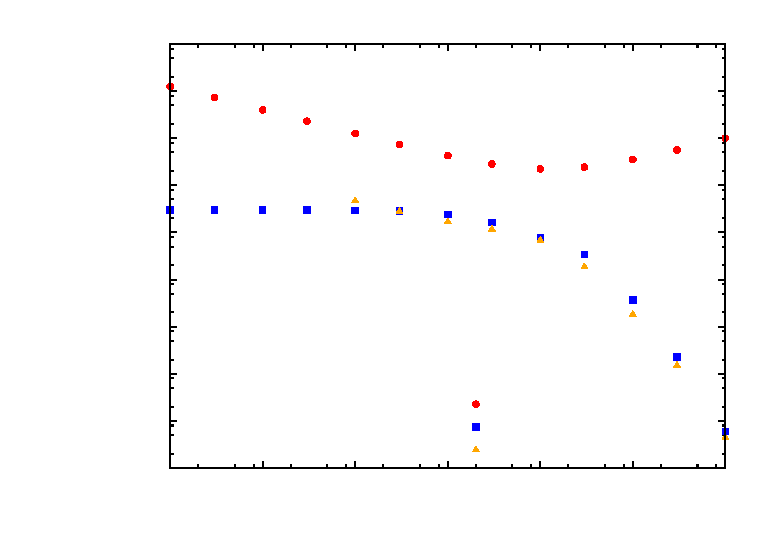
\includegraphics[width=0.61\textwidth]{Figures/water1}
   %\resizebox{\columnwidth}{!}{% GNUPLOT: LaTeX picture with Postscript
\begingroup
  \makeatletter
  \providecommand\color[2][]{%
    \GenericError{(gnuplot) \space\space\space\@spaces}{%
      Package color not loaded in conjunction with
      terminal option `colourtext'%
    }{See the gnuplot documentation for explanation.%
    }{Either use 'blacktext' in gnuplot or load the package
      color.sty in LaTeX.}%
    \renewcommand\color[2][]{}%
  }%
  \providecommand\includegraphics[2][]{%
    \GenericError{(gnuplot) \space\space\space\@spaces}{%
      Package graphicx or graphics not loaded%
    }{See the gnuplot documentation for explanation.%
    }{The gnuplot epslatex terminal needs graphicx.sty or graphics.sty.}%
    \renewcommand\includegraphics[2][]{}%
  }%
  \providecommand\rotatebox[2]{#2}%
  \@ifundefined{ifGPcolor}{%
    \newif\ifGPcolor
    \GPcolortrue
  }{}%
  \@ifundefined{ifGPblacktext}{%
    \newif\ifGPblacktext
    \GPblacktexttrue
  }{}%
  % define a \g@addto@macro without @ in the name:
  \let\gplgaddtomacro\g@addto@macro
  % define empty templates for all commands taking text:
  \gdef\gplbacktext{}%
  \gdef\gplfronttext{}%
  \makeatother
  \ifGPblacktext
    % no textcolor at all
    \def\colorrgb#1{}%
    \def\colorgray#1{}%
  \else
    % gray or color?
    \ifGPcolor
      \def\colorrgb#1{\color[rgb]{#1}}%
      \def\colorgray#1{\color[gray]{#1}}%
      \expandafter\def\csname LTw\endcsname{\color{white}}%
      \expandafter\def\csname LTb\endcsname{\color{black}}%
      \expandafter\def\csname LTa\endcsname{\color{black}}%
      \expandafter\def\csname LT0\endcsname{\color[rgb]{1,0,0}}%
      \expandafter\def\csname LT1\endcsname{\color[rgb]{0,1,0}}%
      \expandafter\def\csname LT2\endcsname{\color[rgb]{0,0,1}}%
      \expandafter\def\csname LT3\endcsname{\color[rgb]{1,0,1}}%
      \expandafter\def\csname LT4\endcsname{\color[rgb]{0,1,1}}%
      \expandafter\def\csname LT5\endcsname{\color[rgb]{1,1,0}}%
      \expandafter\def\csname LT6\endcsname{\color[rgb]{0,0,0}}%
      \expandafter\def\csname LT7\endcsname{\color[rgb]{1,0.3,0}}%
      \expandafter\def\csname LT8\endcsname{\color[rgb]{0.5,0.5,0.5}}%
    \else
      % gray
      \def\colorrgb#1{\color{black}}%
      \def\colorgray#1{\color[gray]{#1}}%
      \expandafter\def\csname LTw\endcsname{\color{white}}%
      \expandafter\def\csname LTb\endcsname{\color{black}}%
      \expandafter\def\csname LTa\endcsname{\color{black}}%
      \expandafter\def\csname LT0\endcsname{\color{black}}%
      \expandafter\def\csname LT1\endcsname{\color{black}}%
      \expandafter\def\csname LT2\endcsname{\color{black}}%
      \expandafter\def\csname LT3\endcsname{\color{black}}%
      \expandafter\def\csname LT4\endcsname{\color{black}}%
      \expandafter\def\csname LT5\endcsname{\color{black}}%
      \expandafter\def\csname LT6\endcsname{\color{black}}%
      \expandafter\def\csname LT7\endcsname{\color{black}}%
      \expandafter\def\csname LT8\endcsname{\color{black}}%
    \fi
  \fi
  \setlength{\unitlength}{0.0500bp}%
  \begin{picture}(7200.00,5040.00)%
    \gplgaddtomacro\gplbacktext{%
      \csname LTb\endcsname%
      \put(1342,704){\makebox(0,0)[r]{\strut{} 1e-05}}%
      \put(1342,1156){\makebox(0,0)[r]{\strut{} 0.0001}}%
      \put(1342,1609){\makebox(0,0)[r]{\strut{} 0.001}}%
      \put(1342,2061){\makebox(0,0)[r]{\strut{} 0.01}}%
      \put(1342,2513){\makebox(0,0)[r]{\strut{} 0.1}}%
      \put(1342,2966){\makebox(0,0)[r]{\strut{} 1}}%
      \put(1342,3418){\makebox(0,0)[r]{\strut{} 10}}%
      \put(1342,3870){\makebox(0,0)[r]{\strut{} 100}}%
      \put(1342,4323){\makebox(0,0)[r]{\strut{} 1000}}%
      \put(1342,4775){\makebox(0,0)[r]{\strut{} 10000}}%
      \put(1474,484){\makebox(0,0){\strut{} 0.001}}%
      \put(2362,484){\makebox(0,0){\strut{} 0.01}}%
      \put(3250,484){\makebox(0,0){\strut{} 0.1}}%
      \put(4139,484){\makebox(0,0){\strut{} 1}}%
      \put(5027,484){\makebox(0,0){\strut{} 10}}%
      \put(5915,484){\makebox(0,0){\strut{} 100}}%
      \put(6803,484){\makebox(0,0){\strut{} 1000}}%
      \put(176,2739){\rotatebox{-270}{\makebox(0,0){\strut{}Intensity [arb. u.]}}}%
      \put(4138,154){\makebox(0,0){\strut{}E$_	ext{kin}$ [eV]}}%
    }%
    \gplgaddtomacro\gplfronttext{%
      \csname LTb\endcsname%
      \put(3982,1317){\makebox(0,0)[r]{\strut{}Coulomb ($|vec{k}|=0$)}}%
      \csname LTb\endcsname%
      \put(3982,1097){\makebox(0,0)[r]{\strut{}spherical}}%
      \csname LTb\endcsname%
      \put(3982,877){\makebox(0,0)[r]{\strut{}Coulomb}}%
    }%
    \gplbacktext
    \put(0,0){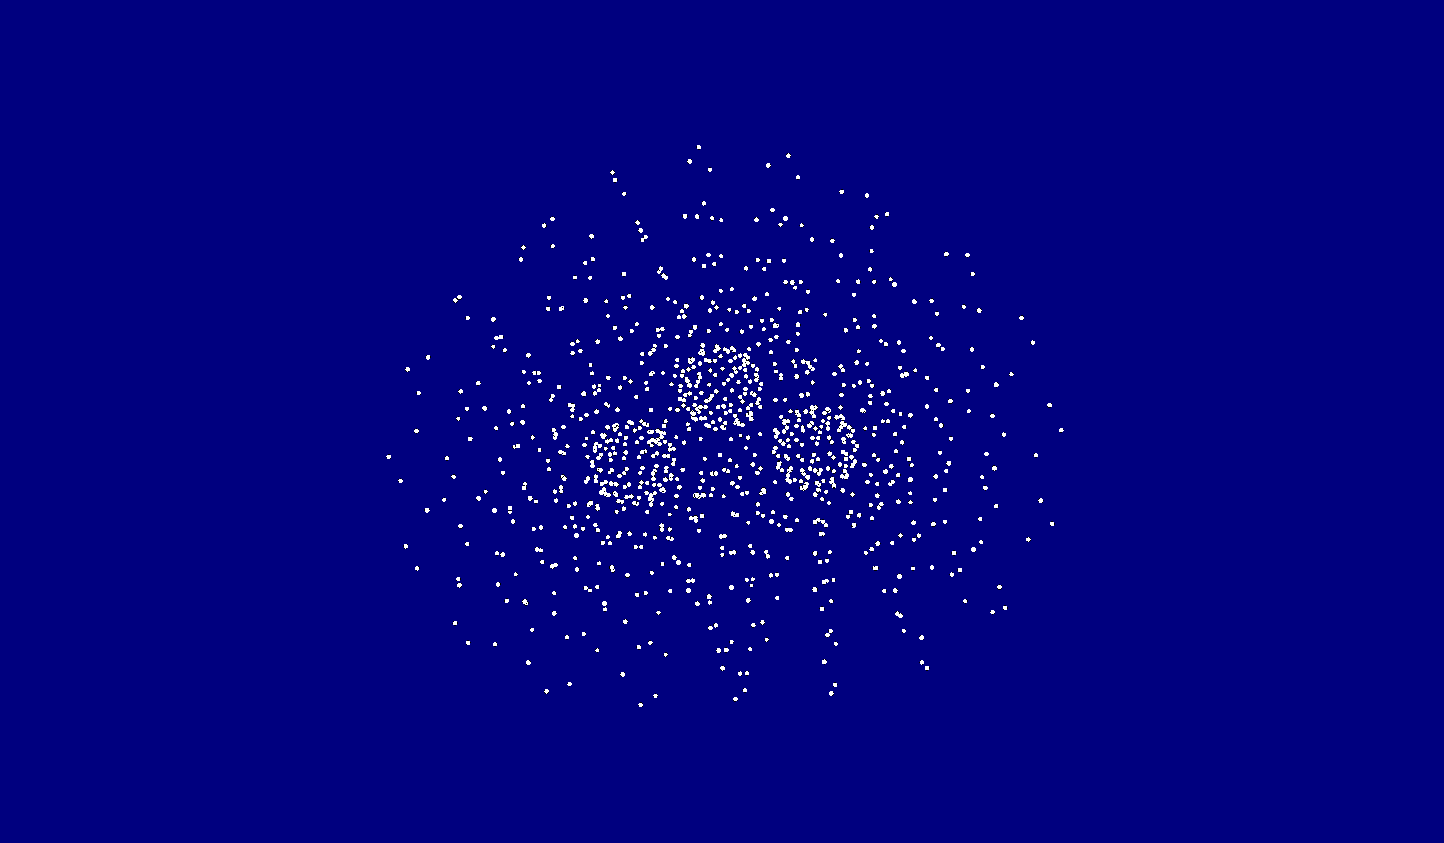
\includegraphics{water1}}%
    \gplfronttext
  \end{picture}%
\endgroup
}
   \caption{The intensity of the lowest-lying transition of water depending on the kinetic energy of the photoelectron. Each expansion is performed up to $l=10$.} 
   \label{fig:Ekin}
\end{wrapfigure}
To overcome the restrictions in symmetry and kinetic energy of the photoelectron function, an explicit formulation is needed, taking the molecular electrostatic potential experienced by the outgoing electron into account.
%To account for the exact electrostatic potential, the final state needs to be treated as a full $N$ electron system to account for the correlation effects.
Assuming that the correlation between the FEF and the bound states of the ion is weak (which is a prerequisit for the DO formalism anyway), one can use the mean-field potential of the molecular remainder.
This allows for obtaining the FEF from the one-electron SE with an appropriate potential and thus reduces the complexity compared to the exact case where a coupled $N$-electron equation needs to be solved, considerably.

In the thesis at hand a good approximation to the FEF is aimed which should be applicable to a wide range of molecules and photon energies.
Such a flexible description is possible exploiting the finite element method for solving the SE.
In the finite element method, the space of interest is subdivided into small volume elements and solved variationally with stepwise polynomials whose support spans over one or few elements only \cite{femBraess,femGilbarg}.
The finite element description is especially efficient here since the size of the elements can be locally adapted to reproduce finer structures or broader shapes \cite{femBraess,femCiarlet}.
Using finite elements, the one-particle SE is formulated a generalised eigenvalue problem with sparse matrices.

An important characteristic of the exact FEF is its spatially infinite extend which can not be handled by the finite element method.
To describe the function in a good approximation, the finite elements are extended by infinite elements \cite{astley3, astley2, Astley,dreyer} which are volume elements with infinite radial extend that are connected to the outer surface of the finite element region.
Thereby the radial function is a polynomial in $\frac 1r$ multiplied by $e^{ikr}$, resembling the asymptotic behaviour of known analytic solutions and fulfilling the Sommerfeld radiation condition \cite{sommerfeldCond}.

%The bound states can be obtained on the level of density functional theory (DFT) which is a formally exact method and yields a quadratic scaling with the number of electrons compared to the exponential growth of the SE \textcolor{green}{source}.
%The DFT is based on the Hohenberg-Kohn theorems \cite{HohenbergKohn}, stating that the total electron density contains all information to obtain any system property.
%However, the correct form of the exchange potential as well as the kinetic energy are not known therein and hence approximate functionals need used.
%While the kinetic energy can be estimated reasonably by the Kohn-Sham scheme \cite{KohnSham}, the expressions used for the exchange-correlation potential yield electron densities that have a wrong long-range asymptotic behaviour which affects the observables of these systems \cite{Koerzd1, Koerzd2, Bokareva}.
%To reduce this error, range-separated hybrid functionals are used where the usual DFT exchange functionals are used at close distances while a Hartree-Fock exact exchange ensures the correct behaviour at larger distances.
%Thereby the interchange between these contributions is modelled via an error function with a characteristic distance that is optimized for each system separately.
%This procedure has been observed to enhance the accuracy of the predicted properties such as the orbital energies \cite{Bokareva,GrellKuehn, Gerber, Gerber2}.
The bound states can be obtained on the level of density functional theory (DFT) which is a formally exact method based on the Hohenberg-Kohn theorem \cite{HohenbergKohn}, stating that the total electron density determines all system properties such as electronic binding energies.
However, the correct form of the exchange potential as well as the kinetic energy are not known as functionals of the electron densety and hence approximate functionals need used.
While the kinetic energy can be estimated reasonably by the Kohn-Sham scheme \cite{KohnSham}, the expressions used for the exchange-correlation potential yield electron densities that have a wrong long-range asymptotic decay which affects the observables of these systems \cite{Koerzd1, Koerzd2, Bokareva}.
To reduce this error, range-separated hybrid functionals are used where the usual DFT exchange functionals are used at small distances while a Hartree-Fock exact exchange ensures the correct behaviour at larger distances.
The interchange between these contributions is modelled via an error function with a characteristic distance that is optimized for each system separately.
This procedure has been observed to enhance the accuracy of the predicted properties such as the orbital energies \cite{Bokareva,GrellKuehn, Gerber, Gerber2}.

While the schemes described above are well established, their combination is only rarely used.
Especially the FEF is found in literature to be approximated only crudely as plane-wave functions \cite{planeWave} or in some expansion as described above \cite{ezDyson,MAgg,GrellKuehn}.
The goal of this thesis is to use the DO formalism with bound states being described by DFT using the above-mentioned optimized range-separated hybrid (OTRSH) functionals to obtain accurate orbital energies and complement it with a FEF that accounts the molecular electrostatic potential explicitly using the finite and infinite element methods which have been applied only to very few quantum mechanical problems \cite{sobaMolecule,bettessHarmonic}.

%The Dyson formalism is well established and has been shown to give reasonable quantitative agreement with experiment for many different systems \cite{ezDyson,DO_TDDFT,bawagan,hafied}.
%In the protocol used the DO is calculated using density functional theory (DFT) and its time-dependent counterpart with a locally modified version of \prog{NWChem} \cite{nwchem} and the \prog{Gaussian 09} package \cite{g09}.
In the protocol used the DFT and time-dependent DFT calculations for excited states are done using a locally modified version of \prog{NWChem} \cite{nwchem} and the \prog{Gaussian 09} package \cite{g09}.
From those, the DO is calculated with the in-house code \prog{DYSON} developed previously \cite{MAgg}.
A self-written interface extracts the required data as \textit{e.g.} the molecular orbital coefficients and overlap matrix of atomic orbitals from the output of these programs.
For the computation of the FEF, the implementation that is developed in the framework of this thesis uses the finite element library \prog{Libmesh} \cite{libmesh}. 
It is an open source library that provides a broad range of capabilities and interfaces to several high-performance linear algebra libraries \cite{slepc1,slepc2,petsc}.
Moreover, it supports MPI parallelisation and implements a recent formulation of the above-mentioned infinite elements \cite{dreyer}.
Especially the latter is to the best of my knowledge a unique option.
Furthermore it has an automated procedure to adaptively refine or coarsen the elements according to local error estimates.

Tho goal of this thesis is to find a systematic way to setup the finite element mesh for any given molecule to describe the photoelectron with a reasonable accuracy that goes beyond the capabilities of existing programs in this field.
%Moreover, the molecular electrostatic potential is to be obtained in the region of interest, requirering some modification in the code of \prog{NWChem} and a three-dimensional interpolation scheme that can handle nonuniform data.
%Finally, to obtain the dipole matrix elements, the DO has to be projected onto the space of finite elements.
%Therfore the explicit function is obtained by evaluating the basis functions at given quadrature points.
\textcolor{red}{
This procedure will be tested on different model systems.
\begin{itemize}
   \item Lithium: light atomic system, many experimental and experimental reference data available, the \prog{ezDyson} calculations are expected to give a good approximation.
   \item CO$_2$: linear easy molecule with some reference data available, used to test some further properties 
   \item Benzene (?): More complex molecule with reference data, well investigated
   \item Some other system(s) for which \prog{ezDyson} gives poor results (?)
\end{itemize}
}
